% Working revision, 2026-09-30. NOT CLEARED FOR SUBMISSION.
% See docs/dmkd_revision_status_2026-09-30.md for version and calendar gates.
% Frozen forecasts are retained; no model was refitted for this revision.
% hyperref is loaded by the sn-jnl class; pass options before \documentclass to avoid option clashes
\PassOptionsToPackage{bookmarksdepth=4}{hyperref}
% The sn-jnl class expects the engine option to correctly configure URL breaking.
\documentclass[pdflatex,sn-mathphys]{sn-jnl}
\usepackage{float}
\usepackage[utf8]{inputenc}
\usepackage[T1]{fontenc}
\usepackage{lmodern}
\usepackage{microtype}
% DMKD figure-caption requirement: bold "Fig." and bold number, no colon
% (avoid caption-package class-detection warnings under sn-jnl)
\makeatletter
\renewcommand{\figurename}{Fig.}
\renewcommand{\fnum@figure}{\textsf{\textbf{\figurename~\thefigure}}}
\makeatother
\usepackage{amsmath,amssymb}
\usepackage{booktabs}
% sn-jnl controls the page layout; avoid overriding margins via geometry.
% \usepackage{geometry}
\usepackage{array}
\usepackage{tabularx}
\usepackage{multirow}
\usepackage{natbib} % ensure natbib is loaded for \setcitestyle
\setcitestyle{aysep={ }} % author-year citations without a comma (e.g., \citep{tashman2000} -> (Tashman 2000)
\usepackage{xurl} % better line breaks for URLs/DOIs (reduces overfull boxes)
\Urlmuskip=0mu plus 1mu
\usepackage{graphicx}
\graphicspath{{figures/}}
% Horizon-descriptor macros
\newcommand{\Hrelax}{$\text{H}^*_{\text{relax}}$}
\newcommand{\Hstrict}{$\text{H}^*_{\text{strict}}$}
% Reduce (or silence) underfull/overfull line warnings without changing wording
\pretolerance=1000
\tolerance=2000
\setlength{\emergencystretch}{3em}
\hbadness=10000
\title[Operational predictability horizons]{Operational Predictability Horizons Under Persistence Baselines}
\author*[1]{Federico Garcia Crespi}
\email{fedeg@umh.es}
\author[2]{Julio Alberto Ramos Martinez}
\email{j.ramos@umh.es}
\affil[1]{Departamento de Ingenier\'ia de Computadores, Universidad Miguel Hern\'andez, Elche, Spain}
\affil[2]{Unidad de Docencia Online de la UMH, Universidad Miguel Hern\'andez, Elche, Spain (T\'ecnico de Innovaci\'on Docente)}
\abstract{Machine learning models for multi-step time series prediction are typically summarized at a few fixed lead times,
which can obscure the practical question of how long a learned model remains useful
relative to an explicit baseline, and whether any benefit is sustained or
only sporadic across the forecast horizon. We recast predictability-horizon
estimation as an evaluation task and measure baseline-relative
performance through the forecast skill curve $\mathrm{Skill}(h)$, obtained
using rolling-origin model fitting with persistence as the
reference. To distinguish total positive reach from sustained contiguous
usefulness, we report two complementary horizon descriptors:
$H^*(\mathrm{relax})$, the last horizon at which $\mathrm{Skill}(h)>0$
(allowing intermediate non-positive gaps), and $H^*(\mathrm{strict})$, the
length of the longest contiguous interval of positive skill, together with
interval locations when profiles are delayed or fragmented. Empirically,
we apply the shared protocol across heterogeneous domains (air quality,
energy, wind, and traffic), and two independent PM$_{10}$ stations (Madrid
and Barcelona, 2017--2024) provide additional descriptive examples, with
Ridge achieving $\text{H}^*_{\text{strict}}=7$ and 85--100\% DM-significant
differences relative to persistence at both sites. These additional results
require qualification of preprocessing and calendar support and do not establish
validated alerting policies. These results suggest that evaluation protocols for ML-based time series prediction should report not only aggregate accuracy but also the structure of baseline-relative usefulness across horizons.}
\keywords{time series evaluation; predictive reach; baseline-relative skill; rolling-origin validation; machine learning benchmarking; multi-step prediction}
\begin{document}
\maketitle

%% ========================================================================
%% §1 INTRODUCTION
%% ========================================================================
\section{Introduction}
In machine learning for time series prediction, model performance is conventionally reported at a small number of fixed lead times. This approach can make it unclear when (and for how long) a trained model is practically advantageous compared to a strong baseline, particularly when multi-step performance varies non-monotonically or is unevenly distributed over the horizon. Methodological audits also document recurrent evaluation failures—including temporally invalid partitioning, leakage-prone preprocessing, omitted parsimonious baselines, and uncritical metric selection—that can materially distort conclusions about practical forecasting value \citep{hewamalage2023dmkd}. Even when leakage is controlled, conventional fixed-horizon summaries and single summary descriptors are not designed to characterise fragmented positive-skill intervals, the delayed emergence of usefulness, or the distinction between total positive reach and sustained contiguous usefulness. As a result, the operational question of \emph{where} and \emph{for how long} a method improves on a clear baseline is not directly answered by common reporting conventions.
We address this capacity gap with rolling-origin evaluation, train-window model preprocessing, and persistence as an explicit reference baseline. Horizon-wise baseline-relative performance is reported as skill curves $\mathrm{Skill}(h)$. Historical input cleaning and calendar alignment are separate validity requirements; the limitations of the retained artifacts are stated explicitly below.
Operational reach is then summarised using complementary horizon descriptors that separate total positive reach from sustained contiguous usefulness. Specifically, we report $H^*(\mathrm{relax})$ and $H^*(\mathrm{strict})$, along with interval locations and sign-change structures when profiles are fragmented or delayed, to make horizon continuity and fragmentation explicit.
This evaluation-methodology framing complements recent work on evaluation pitfalls and multi-step forecasting in machine learning and data mining \citep{hewamalage2023dmkd,green2025stratify,kreuzer2025trend,cerqueira2020,modelradar2025}.
Empirically, we examine six stored domain evaluations—PM$_{2.5}$ air quality, electric load, wind speed, traffic speed, and PM$_{10}$ at two Spanish urban stations (Madrid Casa de Campo and Barcelona Eixample, 2017–2024). They span heterogeneous dynamics and baseline competitiveness, but calendar and historical input-preparation defects prevent claiming a uniformly verified protocol across all six.
The paper makes three contributions:
\begin{enumerate}
  \item \textbf{A reproducible baseline-relative evaluation framework:} we specify a rolling-origin protocol with train-window model preprocessing that computes horizon-wise skill $\mathrm{Skill}(h)$ relative to an explicit persistence baseline. Full temporal validity additionally requires verified causal input preparation and calendar support.
  \item \textbf{Operational horizon descriptors for useful predictive reach and continuity:} we instantiate the generic predictability-horizon concept via two complementary descriptors—$H^*(\mathrm{relax})$, the maximum evaluated horizon such that $\mathrm{Skill}(h)>0$ (allowing intermediate non-positive gaps), and $H^*(\mathrm{strict})$, the length of the longest contiguous positive-skill interval $[h_{\mathrm{start}},h_{\mathrm{end}}]$—augmented, when needed, with interval locations and sign-change structure for fragmented or late-recovery profiles.
  \item \textbf{A cross-domain empirical analysis under a shared protocol:} we show that domains differ not only in positive reach but also in continuity and fragmentation, including cases of descriptor preservation under protocol-matched model substitution and cases where relaxed reach is stable, but contiguous usefulness is model-sensitive.
\end{enumerate}
Together, these contributions provide a baseline-relative basis for describing operational predictability horizons, subject to explicit temporal-validity checks.

%% ========================================================================
%% §2 RELATED WORK
%% ========================================================================
\section{Related Work}
\subsection{Forecast evaluation metrics}
Within the forecasting literature, forecast evaluation is most often framed in terms of
accuracy metrics such as MAE and RMSE, along with scaled or relative variants that enable
comparisons across different series and applications. \citet{hyndman2006} surveys
the most commonly used measures and underscores that no single metric is universally ideal;
the appropriate choice depends on scale, loss asymmetry, and the decisions the forecasts are
intended to inform \citep{petropoulos2022}.
For probabilistic forecasts, evaluation is commonly grounded in strictly proper scoring rules,
which ensure that the expected score is optimised by the forecaster's true predictive
distribution \citep{gneiting2007}. This framework shifts the evaluation focus from
point accuracy to the full predictive distribution, but the predominant empirical convention
remains point-forecast-based reporting at fixed horizons.
When comparing forecasting methods, statistical tests of predictive accuracy (e.g., the
Diebold–Mariano framework) are also frequently used to assess whether observed differences
are larger than would be expected by chance \citep{diebold1995}. In this work, horizon-wise
skill is reported relative to persistence and is complemented with formal horizon-wise
significance testing using the Harvey--Leybourne--Newbold modified Diebold--Mariano test
\citep{harvey1997} with Benjamini--Hochberg false-discovery-rate correction \citep{benjamini1995}.
Empirical work typically reports errors for one or a few fixed horizons. While convenient, this fixed-horizon focus can hide how performance changes with lead time, including non-monotonic, fragmented, or delayed skill profiles in multi-step settings. Operationally, it can therefore be unclear whether a method is unhelpful overall or whether it provides baseline-relative usefulness only over specific horizon intervals. Fixed-horizon reporting also makes it difficult to directly identify where horizon-wise skill becomes non-positive relative to an explicit baseline.
Large-scale benchmark exercises have reinforced this convention.
Comparisons such as the M4 competition \citep{makridakis2020} and
repositories like the Monash Time Series Forecasting Archive
\citep{godahewa2021} assess many methods over many series, but usually
at fixed or pre-chosen horizons. This setup is effective for contrasting
methods on relative accuracy; yet, it does not directly characterize
how forecast skill evolves over the full horizon range or at which point
baseline-relative skill is exhausted.
A further drawback of fixed-horizon summaries is that, even when a
strong baseline is available, they only indirectly address operational
relevance. From an applied standpoint, the key question is often not
whether a method lowers error at a single, predefined horizon, but
whether it consistently improves on a baseline across the set of
horizons that matter for planning, control, or service-level agreements.
\citet{hyndman2018} consolidates prevailing guidance on forecast
evaluation and highlights the need for out-of-sample validation and for
matching the evaluation design to how forecasts are generated and used.
This points to evaluation constructs that summarize performance over
horizons and that are interpretable relative to a clearly specified
reference forecast.
Related methodological audits emphasize that common evaluation pitfalls (e.g., leakage-prone splits and missing strong baselines) can materially distort conclusions about practical forecasting value \citep{hewamalage2023dmkd}; we use this as motivation for the leakage-free, baseline-relative protocol described in Section~\ref{sec:framework}.
\subsection{Forecast skill evaluation}
Baseline-relative evaluation is often expressed in terms of forecast
skill, which measures the error of a candidate forecasting method
against that of a reference forecast:
\begin{equation}
\mathrm{Skill}(h) = 1 - \frac{E_{\mathrm{model}}(h)}{E_{\mathrm{baseline}}(h)}.
\end{equation}
This representation is fundamental in forecast verification, where the
quality of a forecast is defined only in relation to a baseline
\citep{murphy1993}. In practical forecasting settings, the same rationale
underpins operational interpretation: a model that marginally improves
absolute error may still be operationally unimportant if it does not
surpass a strong baseline at the horizons that matter, whereas a model
whose gains appear only after a period of short-horizon baseline
dominance can still be highly useful for longer-range decision-making.
Skill-based reporting aligns naturally with multi-horizon evaluation
because it produces a horizon-specific quantity, the skill curve
$\mathrm{Skill}(h)$, instead of a single aggregate metric. This
facilitates distinguishing between evaluation outcomes driven by the
strength of the baseline and those stemming from modeling decisions. It
also underscores the importance of rigorous temporal evaluation
protocols. Out-of-sample forecast tests are typically implemented via
time-aware designs such as rolling-origin evaluation, which repeatedly
re-fits models and scores forecasts as the forecast origin moves forward
in time \citep{tashman2000}. These designs mirror real forecasting
practice and mitigate the risk that conclusions hinge on a particular
train--test split. The suitability of rolling-origin designs, in
contrast to blocked or random cross-validation for time series, has been
investigated empirically, with evidence indicating that respecting
temporal order is crucial for reliable performance estimation
\citep{cerqueira2020, bergmeir2012}.
In machine-learning-based forecasting, this principle is coupled with a
further practical issue: preventing temporal leakage arising from
preprocessing, feature engineering, hyperparameter tuning, or validation
procedures that inadvertently exploit future information~\citep{kapoor2023leakage}. Such leakage
can artificially boost apparent skill, especially at short horizons where
persistence effects are strong and where small misalignments or
preprocessing-related leakage can dominate evaluation results. Therefore,
leakage-free temporal validation is essential for interpreting skill
curves and for using baseline-relative evaluation to draw operational
conclusions about when forecasts are genuinely beneficial.
\subsection{Predictability limits}
Finite predictability in complex systems has long been recognized as a
core issue in forecasting and dynamical systems. \citet{lorenz1969}
demonstrated that sensitivity to initial conditions can create inherent
constraints on the lead times over which accurate prediction is
achievable. In empirical forecasting, similar limitations appear as the
horizon grows and the baseline becomes increasingly difficult to surpass.
However, these limits are not solely characteristics of a particular
model class; they emerge from the interplay among the system's dynamics,
the choice of reference forecast, and the evaluation protocol.
Fixed-horizon accuracy metrics remain the dominant reporting convention~\citep{makridakis2020,godahewa2021},
but they do not directly identify the horizon at which baseline-relative
skill is exhausted. From an operational standpoint, the key quantity is
the range of horizons over which a method achieves positive skill
relative to a baseline, under a clearly specified, temporally coherent
evaluation design.
A further limitation is comparability across heterogeneous domains.
Although baseline-relative skill measures are well established
\citep{hyndman2006, murphy1993, tashman2000}, the literature less
frequently provides cross-domain descriptions of practically useful
predictability horizons under a shared, leakage-free protocol. Large
benchmark studies \citep{makridakis2020, godahewa2021} compare methods
based on accuracy, but typically do not interpret the results as
operational estimates of when baseline-relative skill is depleted.
Without such a shared protocol, it remains unclear whether differences in
reported predictability across domains reflect genuine differences in system
dynamics and baseline competitiveness, or merely reflect inconsistencies in
evaluation design, preprocessing choices, or baseline specification.
This gap motivates baseline-relative horizon descriptors that summarize
the span of positive skill in a way that is robust to fragmented or
slowly emerging skill profiles and that supports comparison across
forecasting systems without conflating predictability with
methodological novelty or dataset-specific tuning.

%% ========================================================================
%% §3 PROBLEM FORMULATION
%% ========================================================================
\section{Problem Formulation}
Consider a time series $y_t$, $t = 1,\dots,T$.
A forecasting model generates predictions
\begin{equation}
\hat{y}_{t+h} = f_{\theta}(y_t, \dots, y_{t-L+1}),
\end{equation}
where $L$ denotes the input window length and $h$ the forecast horizon.
The corresponding forecast error is
\begin{equation}
e_{t,h} = y_{t+h} - \hat{y}_{t+h}.
\end{equation}
An aggregated error measure at horizon $h$ is given by $E(h)$, for
example, MAE or RMSE. A baseline forecasting method $b(\cdot)$ induces
a baseline error curve $E_{\mathrm{baseline}}(h)$.
\subsection{Operational Predictability Horizon}
In this work, operational predictability is understood as the range of time over which a forecasting system maintains positive skill relative to an explicit baseline, under a fixed, leakage-free evaluation setup.
We use $H^*$ as the generic conceptual notation for the operational predictability horizon: the maximum forecast horizon at which a model maintains positive skill relative to an explicit baseline under a specified evaluation protocol. Formally, the generic \emph{Forecast Skill Horizon} is
\begin{equation}
  H^* = \max \left\{ h \in \mathcal{H} : \mathrm{Skill}(h) > 0 \right\},
  \qquad
  \mathrm{Skill}(h) = 1 - \frac{E_{\mathrm{model}}(h)}{E_{\mathrm{baseline}}(h)}.
\end{equation}
Here, $\mathcal{H}$ denotes the set of evaluated forecast horizons. $H^*$ is protocol-defined: its value depends on the baseline choice (persistence in this work), preprocessing strategy, error metric, and evaluation scheme (leakage-free rolling-origin). This dependency is intentional, as it makes the descriptor reproducible and operationally interpretable.
\subsubsection{Operational definitions}
In empirical multi-step settings, $\mathrm{Skill}(h)$ curves may be
non-monotonic, fragmented, or exhibit delayed recovery, so the single
generic definition above is best treated as a conceptual anchor.
For example, a curve with early negative skill but a late positive
recovery yields a large $H^*(\mathrm{relax})$ but a short
$H^*(\mathrm{strict})$—two descriptors that a single maximum-horizon
summary conflates.
We therefore instantiate $H^*$ through two complementary reported
descriptors, defined over the evaluated horizon set
$\mathcal{H} = \{1, 2, \dots, H_{\max}\}$ and the positive-skill
subset $\mathcal{H}^+ = \{h \in \mathcal{H} \mid \mathrm{Skill}(h) > 0\}$. In the remainder of the paper, $H^*$ is used as the generic conceptual label for the operational predictability horizon, whereas all empirical reporting is based on the two instantiated descriptors $H^*(\mathrm{relax})$ and $H^*(\mathrm{strict})$.
\textbf{$H^*(\mathrm{relax})$:} The relaxed horizon is the maximum
evaluated horizon such that $\mathrm{Skill}(h)>0$, allowing intermediate
horizons with non-positive skill.
\begin{equation}
  \begin{aligned}
  H^*(\mathrm{relax}) &= \max\!\bigl(\mathcal{H}^+ \cup \{0\}\bigr),\\
  \mathcal{R}_{\mathrm{relax}} &= \{1,\ldots,H^*(\mathrm{relax})\},\qquad
  \mathcal{R}_{\mathrm{relax}}\setminus\mathcal{H}^+
  =\{h\in\mathcal{R}_{\mathrm{relax}}:\mathrm{Skill}(h)\leq0\}.
  \end{aligned}
\end{equation}
The relaxed span is empty when $H^*(\mathrm{relax})=0$. It includes all
evaluated steps up to the last positive-skill endpoint, including possible
non-positive gaps; those gaps are not themselves labelled useful. Thus a
delayed PM$_{2.5}$ profile or a fragmented Traffic profile can have a large
relaxed endpoint despite persistence dominance at many earlier steps.
\textbf{$H^*(\mathrm{strict})$:} To capture sustained usefulness, let
$\mathcal{I}$ be the collection of all contiguous integer intervals
$I=[h_{\mathrm{start}},h_{\mathrm{end}}]$ with $I\subseteq\mathcal{H}^+$.
The strict horizon is the \emph{length} of the longest such interval:
\begin{equation}
  H^*(\mathrm{strict}) = \max\!\bigl(\{|I|:I\in\mathcal{I}\}\cup\{0\}\bigr),
  \qquad |I| = h_{\mathrm{end}} - h_{\mathrm{start}} + 1.
\end{equation}
We additionally report the maximizing interval location
$[h_{\mathrm{start}}, h_{\mathrm{end}}]$ and, for fragmented or
late-recovery profiles, the full sign-change structure of
$\mathrm{Skill}(h)$. Ties are resolved by reporting the earliest maximizing
interval. A conversion to elapsed time is valid only when the input grid is
regular and target timestamps have been checked; an observation-index interval
must not automatically be interpreted as a calendar-time interval.
Together, these two descriptors distinguish total positive reach from
sustained contiguous usefulness — a distinction that matters in the
fragmented and delayed-onset domains studied below. Fig.~\ref{fig:hstar_conceptual}
provides a conceptual illustration.
\begin{figure}[t]
  \centering
  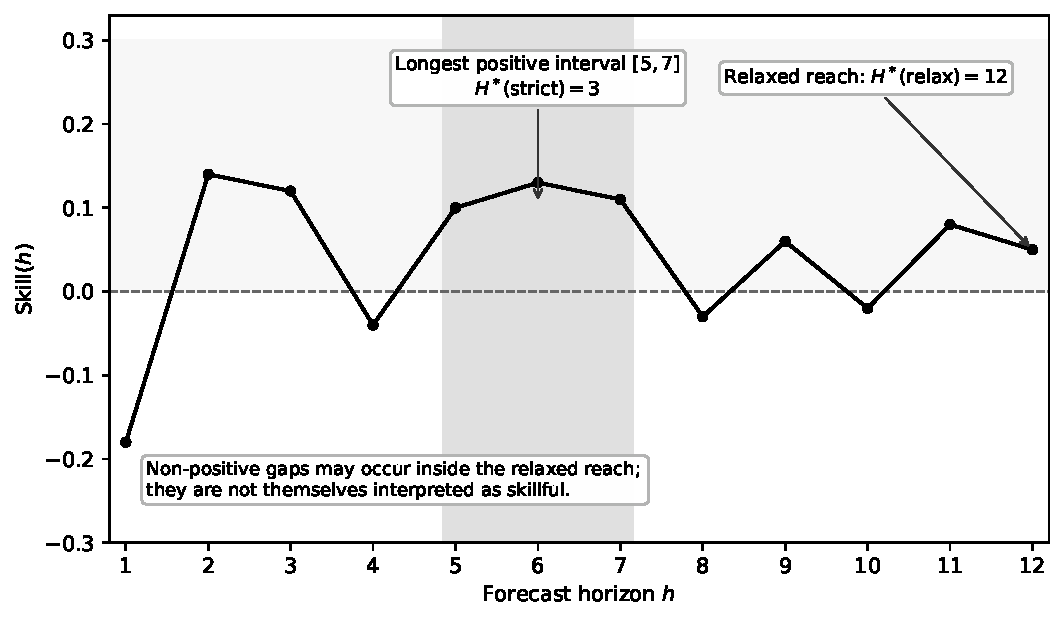
\includegraphics[width=0.7\textwidth]{fig_hstar_conceptual}
  \caption{Conceptual illustration of a baseline-relative skill curve $\mathrm{Skill}(h)$ with both positive and negative regions. The relaxed horizon $H^*(\mathrm{relax})$ is the maximum evaluated horizon with $\mathrm{Skill}(h) > 0$, whereas the strict horizon $H^*(\mathrm{strict})$ is the length of the longest contiguous positive-skill interval $[h_{\mathrm{start}},h_{\mathrm{end}}]$.}
  \label{fig:hstar_conceptual}
\end{figure}

%% ========================================================================
%% §4 EVALUATION FRAMEWORK
%% ========================================================================
\subsection{Operational interpretation and actionability}\label{sec:actionability}
The relaxed descriptor answers how far any positive baseline-relative skill
reaches. It does not justify using the model at every earlier horizon. The
strict descriptor, together with its interval location, identifies the longest
continuous positive-skill window. For example, the Traffic LightGBM interval
$[64,67]$ indicates a four-hour window, not continuous usefulness over all
72 hours. A fixed-horizon or average-error summary does not convey delayed
onset, intervening gaps, or the location and length of that window.

A practitioner should first specify the target, baseline, decision loss and
relevant horizon range, estimate the full skill curve on historical validation
data, and inspect both gain magnitude and uncertainty before choosing any
operational window. Positive average skill alone does not demonstrate the
value or safety of a deployment decision. For adaptive use, a horizon policy
may be estimated from past validation errors and frozen for later forecasts;
updates must use only errors whose targets have already been observed.
Estimating the descriptors, selecting horizons and scoring that selection on
the same errors creates adaptive selection bias. A dynamic policy therefore
requires separate prospective, prequential or nested validation. Such a
controller is a potential application and is not evaluated in this study.

\section{Evaluation Framework}\label{sec:framework}
This section specifies the evaluation components used to compute horizon-wise baseline-relative skill curves $\mathrm{Skill}(h)$ and the associated horizon descriptors: the reference baseline, error metrics, and the leakage-free rolling-origin validation protocol.
\subsection{Baseline models}
In every domain, we evaluate models against a persistence baseline. At forecast origin $t$, the baseline prediction for horizon $h$ is simply the most recent observation available at time $t$. Persistence is intentionally adopted as a strong operational reference because it is easy to implement, transparent, and often highly competitive for short lead times~\citep{murphy1993,hyndman2018}. Accordingly, the evaluation objective is not just to report absolute error levels but to determine the horizons at which a forecasting method yields positive skill relative to this baseline.
For a supplementary sensitivity analysis on verified regular grids, we also
use seasonal persistence,
\begin{equation}
\hat y^{\mathrm{season}}_{t+h}=y_{t+h-\lceil h/s\rceil s},
\end{equation}
with $s=24$ hours for Wind and Traffic and $s=7$ days for Load. The source
index is always at or before the origin. Periods were fixed before this
diagnostic was computed. Existing model forecasts, targets and evaluation
rows are reused without refitting or dropping records. Calendar sensitivity
for irregular inputs is not inferred from row-based seasonal offsets.
\subsection{Evaluation metrics}
Forecast errors are evaluated primarily using mean absolute error (MAE) \citep{hyndman2006}, which serves as the basis for computing baseline-relative skill at each horizon. Root mean squared error (RMSE) is additionally reported as a complementary error measure, but the main operational analysis throughout this work is framed in terms of $\mathrm{Skill}(h)$ computed from MAE. This design choice ensures that horizon-specific comparisons remain straightforward to interpret: at each lead time, we can directly assess whether a given forecasting approach improves upon persistence. A metric-sensitivity analysis based on RMSE-derived skill curves, conducted under the same rolling-origin protocol and persistence baseline, is reported in Appendix~A.1.
\subsection{Temporal validation protocol}
The tabular experiments use rolling-origin model fitting and train-window
scaling with persistence as the reference. This controls model-fitting
leakage but does not by itself verify historical cleaning or calendar
alignment. The limitations below distinguish those outstanding input checks.
Fig.~\ref{fig:rolling_origin} summarizes the intended protocol.
\begin{figure}[t]
  \centering
  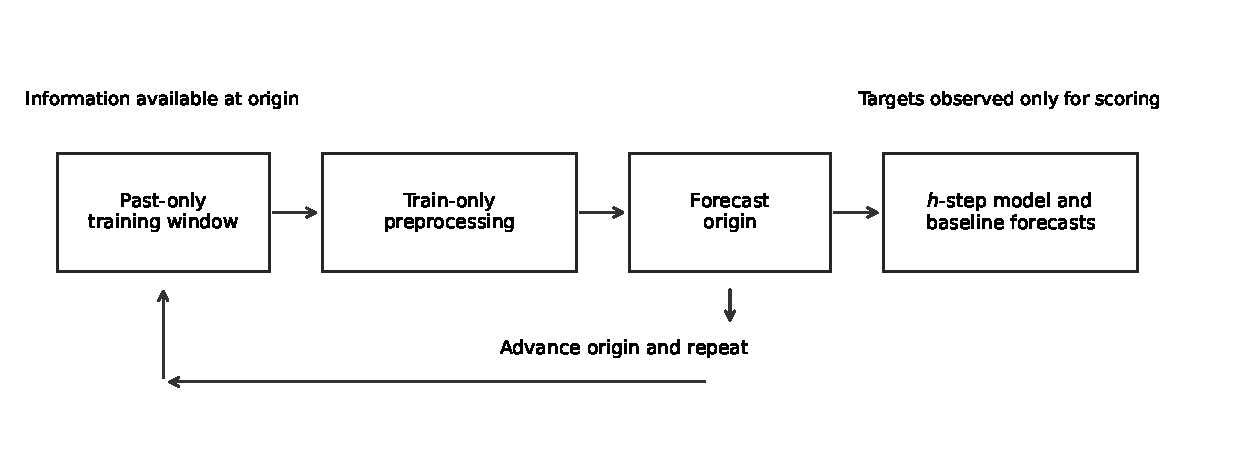
\includegraphics[width=0.75\textwidth]{fig_rolling_origin_protocol}
  \caption{Schematic of the leakage-free rolling-origin evaluation protocol. Each origin uses a past-only training window with train-only preprocessing, generates $h$-step-ahead forecasts for the model and the persistence baseline, and then rolls the origin forward in time.}
  \label{fig:rolling_origin}
\end{figure}
Model fitting is time-ordered. The intended end-to-end protocol adopts a rolling-origin framework~\citep{tashman2000}:
\begin{enumerate}
  \item define a chronologically ordered training window,
  \item fit any preprocessing steps using training data only,
  \item produce model and persistence forecasts for horizon $h$,
  \item advance the forecasting origin,
  \item iterate over all horizons and origins.
\end{enumerate}
Random train-test splits are intentionally avoided because they may introduce temporal leakage.
For all domains, model and baseline forecasts are generated and compared only at aligned timestamps.
\subsection{Horizon-wise significance testing}
To complement descriptive skill profiles, horizon-wise differences in predictive accuracy between each model and persistence were tested using the Harvey--Leybourne--Newbold modified Diebold--Mariano test \citep{harvey1997}. The test was applied two-sided at each horizon for each model, using the rolling-origin loss differentials implied by MAE. The stored Benjamini--Hochberg adjustments use historical domain/model batches; the primary three-model batch and later KNN/MLP batch were adjusted separately. Thus the reported decisions do not establish joint false-discovery control over the entire expanded study. The ``\% DM sign.'' field counts two-sided rejections, including significant deterioration; direction must be read jointly with the sign of skill. Undefined test statistics are not interpreted as evidence of equality. Stored decisions are retained for traceability rather than recomputed during editorial revision.

%% ========================================================================
%% §5 DATASETS AND EXPERIMENTAL SETUP
%% ========================================================================
\section{Datasets and Experimental Setup}\label{sec:setup}

\subsection{Datasets}
Table~\ref{tab:datasets} provides an overview of the application
domains, datasets, target variables, temporal resolution, and maximum
forecast horizon.
The six domains are selected to support methodological comparison under a
shared evaluation design rather than to provide exhaustive
coverage of forecasting applications. They span heterogeneous temporal
structures, differ markedly in baseline competitiveness against
persistence, and vary in temporal resolution and operational context
(hourly environmental and mobility signals versus daily energy and PM$_{10}$
air-quality series). Together, they form a diverse
cross-domain testbed for studying horizon-wise baseline-relative skill and
its operational summaries.
Under this shared protocol, the domains yield distinct baseline-relative
skill-profile morphologies, enabling the comparison of operational reach,
contiguous usefulness, and (when present) fragmented interval structure.
\begin{table}[t]
\centering
\scriptsize
\setlength{\tabcolsep}{2.8pt}
\renewcommand{\arraystretch}{1.12}
\begin{tabularx}{\linewidth}{@{}>{\raggedright\arraybackslash}p{2.3cm} >{\raggedright\arraybackslash}p{3.0cm} >{\centering\arraybackslash}p{1.4cm} r >{\centering\arraybackslash}p{1.0cm} r >{\centering\arraybackslash}p{1.0cm}@{}}
\toprule
Domain & Station / ID & Period & $N$ & Freq. & Eval.\ origins & $H_{\max}$ \\
\midrule
PM$_{2.5}$ (Beijing) & Beijing US Embassy & 2010--2014 & 41{,}757 & Observed rows & 365 & 48 steps \\
Electric Load (UCI) & Aggregate (370 clients) & 2013--2015 & 667 & Daily & 275--281 & 7 days \\
Wind (NREL) & Site 1673080, 100 m & 2019 & 8{,}760 & Hourly & 350--352 & 48 h \\
Traffic (METR-LA) & Sensor 773869 & 2012 & 2{,}856 & Hourly & 102--105 & 72 h \\
PM$_{10}$ Madrid & Casa de Campo & 2017--2024 & 2{,}922 & Daily & 2{,}530--2{,}536 & 7 days \\
PM$_{10}$ Barcelona & Eixample (08019043) & 2017--2024 & 2{,}827 & Observed days & 2{,}435--2{,}441 & 7 steps \\
\bottomrule
\end{tabularx}
\caption{Datasets used for cross-domain predictability analysis. Data sources are described in the corresponding domain results; this table focuses on station/ID, period, sample size $N$, sampling frequency, the number of evaluation origins used in rolling-origin scoring, and the maximum evaluated horizon.}
\label{tab:datasets}
\end{table}
In the traffic domain, the raw source variable corresponds to METR-LA
sensor speed measurements \citep{li2018dcrnn}.

\subsubsection{Data representation}
For each domain, the stored input is univariate. PM$_{2.5}$ is a one-column
sequence with missing raw observations removed; its timestamps were recovered
by exact comparison with the observed raw subsequence for the revision audit.
Barcelona contains only available observation dates and is not a complete
daily grid. In the electric-load domain, the cleaned
representation is $(\texttt{timestamp}, \texttt{value})$ at daily
resolution. The aggregate series is defined as the daily sum of all
available client-level series from the stable-coverage start date
onwards. This explicit specification of the aggregation procedure
specifies the stored scale. Coverage of the final aggregate day and historical
PM$_{10}$ imputation require separate verification.

\subsection{Forecast horizons}
The maximum forecast horizons are chosen to balance practical
operational relevance with a sufficient length to capture the onset and
progression of skill decay:
\begin{itemize}
  \item PM$_{2.5}$ (observation-index input): $H_{\max}=48$ steps,
  \item Electric load (daily): $H_{\max}=7$,
  \item Wind (hourly): $H_{\max}=48$,
  \item Traffic (hourly): $H_{\max}=72$,
  \item PM$_{10}$: $H_{\max}=7$ days for the regular Madrid grid and
  7 observation steps for the irregular Barcelona input.
\end{itemize}
The evaluated ranges differ across domains. No common 48-step calendar-time
range exists across hourly and daily inputs. Numerical horizon lengths must
therefore be interpreted with their domain-specific frequency and support.
\subsection{Models}
Five forecasting models were evaluated against persistence in every domain:
Ridge regression, LightGBM~\citep{ke2017lightgbm}, ExtraTrees, KNN and MLP.
Ridge used a \texttt{StandardScaler} followed by $\alpha=1$ linear regression;
LightGBM used 50 trees, learning rate 0.1 and 31 leaves; ExtraTrees used 50
estimators. KNN used five Euclidean neighbours with uniform weights. MLP used
hidden layers $(64,32)$, ReLU, Adam, a maximum of 500 iterations and early
stopping with a 0.1 validation fraction. Ridge, KNN and MLP scaling was fitted
inside each rolling training window. MLP's internal validation samples are
drawn only from that training window; the target was left unscaled.
These three learners were selected as representatives of distinct learning classes rather than as a model-selection exercise. Ridge represents regularised linear learning with explicit capacity control; LightGBM represents sequential additive learning via gradient-boosted decision trees; and ExtraTrees represents a parallel ensemble with randomised splits and feature subsampling. This coverage makes the learning component explicit and allows differences in $\mathrm{Skill}(h)$ morphology to be understood in terms of inductive bias and bias--variance trade-offs, rather than only in terms of domain difficulty.
All forecasts were generated with a direct multi-step strategy: a separate model was trained for each horizon $h$. At each rolling origin $t_0$, lag features were constructed exclusively from values at or before $t_0$.
Lag/stride settings were aligned with domain frequency. For hourly domains, lags were drawn from short-term and daily-cycle offsets (e.g., including lag 0 so that the model and baseline share the same information at the origin). For daily PM$_{10}$, the setup used horizons $h=1,\ldots,7$ days, lags $\{0,1,2,3,7,14\}$, stride of 1 day, and a minimum training window of 365 days.
The persistence baseline was defined as the most recent observed value available at the prediction origin.
\begin{equation}
\hat{y}^{\mathrm{base}}_{t+h} = y_{t},
\end{equation}
and was applied uniformly in all domains.
No hyperparameter tuning was carried out. The protocol was kept deliberately simple so that observed differences in skill reflect domain characteristics and baseline competitiveness rather than aggressive model optimisation.
% Table 2: Baseline definition in each domain
\begin{table}[t]
\centering
\scriptsize
\setlength{\tabcolsep}{4pt}
\renewcommand{\arraystretch}{1.15}
\begin{tabularx}{\linewidth}{@{}l l >{\raggedright\arraybackslash}X >{\raggedright\arraybackslash}X@{}}
\toprule
Domain / target unit & Baseline & Mathematical / ML definition & Illustrative explanation \\
\midrule
PM$_{2.5}$ ($\mu$g m$^{-3}$) & Persistence &
  Last observation carried forward: $\hat{y}^{\mathrm{base}}_{t+h} = y_t$. &
  If $y_t = 42$~$\mu$g m$^{-3}$, every lead uses 42~$\mu$g m$^{-3}$. \\
Load (stored aggregate) & Persistence &
  Last observation carried forward: $\hat{y}^{\mathrm{base}}_{t+h} = y_t$. &
  Sum of client 15-minute kW readings per day. Dividing by four gives daily energy in kWh. \\
Wind (m s$^{-1}$) & Persistence &
  Last observation carried forward: $\hat{y}^{\mathrm{base}}_{t+h} = y_t$. &
  If $y_t = 6.8$~m s$^{-1}$, every lead uses 6.8~m s$^{-1}$. \\
Traffic (mph) & Persistence &
  Last observation carried forward: $\hat{y}^{\mathrm{base}}_{t+h} = y_t$. &
  If $y_t = 57$~mph, every lead uses 57~mph. \\
PM$_{10}$ ($\mu$g m$^{-3}$) & Persistence &
  Last observation carried forward: $\hat{y}^{\mathrm{base}}_{t+h} = y_t$. &
  If $y_t = 26$~$\mu$g m$^{-3}$, every lead uses 26~$\mu$g m$^{-3}$. \\
\bottomrule
\end{tabularx}
\caption{Persistence definition and target units. Electric load retains the exact stored scale of the historical aggregation; it is not a daily mean in MW. The kWh conversion follows UCI's 15-minute kW convention. No experimental values were rescaled.}
\label{tab:baselines}
\end{table}

Historical ARIMA$(2,0,0)$ artifacts are retained in the replication audit but
excluded from the revised empirical comparison. No documented ACF/PACF or
validation-based rationale establishes why order two was selected, and its
forecast origins differ from those of the tabular experiments. We therefore
do not use these artifacts to support matched-model robustness or invent a
retrospective order-selection rationale.
\subsection{Reproducibility rules}
All tables and figures are generated directly from the experiments
carried out under the stated evaluation protocol. To support
replication, the data-processing and evaluation scripts operate on the
cleaned, domain-specific datasets, with each step documented so that
the reported results can be reproduced from the specified inputs.

%% ========================================================================
%% §6 RESULTS
%% ========================================================================
\section{Results}\label{sec:results}

\subsection{\texorpdfstring{PM$_{2.5}$}{PM2.5} domain}\label{sec:pm25}

\subsubsection{Experimental setting}
The Beijing PM$_{2.5}$ input \citep{chen2015beijingpm25} illustrates delayed
positive skill in the stored sequence. The raw observations are hourly, but
the evaluated input removes missing rows. Its $H_{\max}=48$ is therefore an
observation-index range, not a verified 48-hour range. The numerical results
below are retained as descriptive sequence diagnostics pending calendar repair.

\subsubsection{Observed skill behavior}
For PM$_{2.5}$, the skill curves are delayed and become positive only after an extended short-horizon region dominated by persistence (Fig.~\ref{fig:skill-pm25}). Under this setting, all three models achieve $H^*(\mathrm{relax})=48$, but strict continuity differs substantially: Ridge attains $H^*(\mathrm{strict})=40$ with $[h_{\mathrm{start}},h_{\mathrm{end}}]=[9,48]$, LightGBM attains $H^*(\mathrm{strict})=19$ with $[30,48]$, and ExtraTrees attains $H^*(\mathrm{strict})=26$ with $[23,48]$ (Table~\ref{tab:results}).

\subsubsection{Interpretation}
These outcomes indicate that, in the stored PM$_{2.5}$ observation sequence, baseline-relative usefulness can emerge late but then persist for a long interval; however, the degree of contiguity is model-dependent. Ridge achieves the longest sustained improvement window, while the tree-based models show more fragmented or delayed contiguous usefulness, consistent with persistence being highly competitive at short observation leads. These are not verified calendar-hour intervals.
\begin{figure}[t]
  \centering
  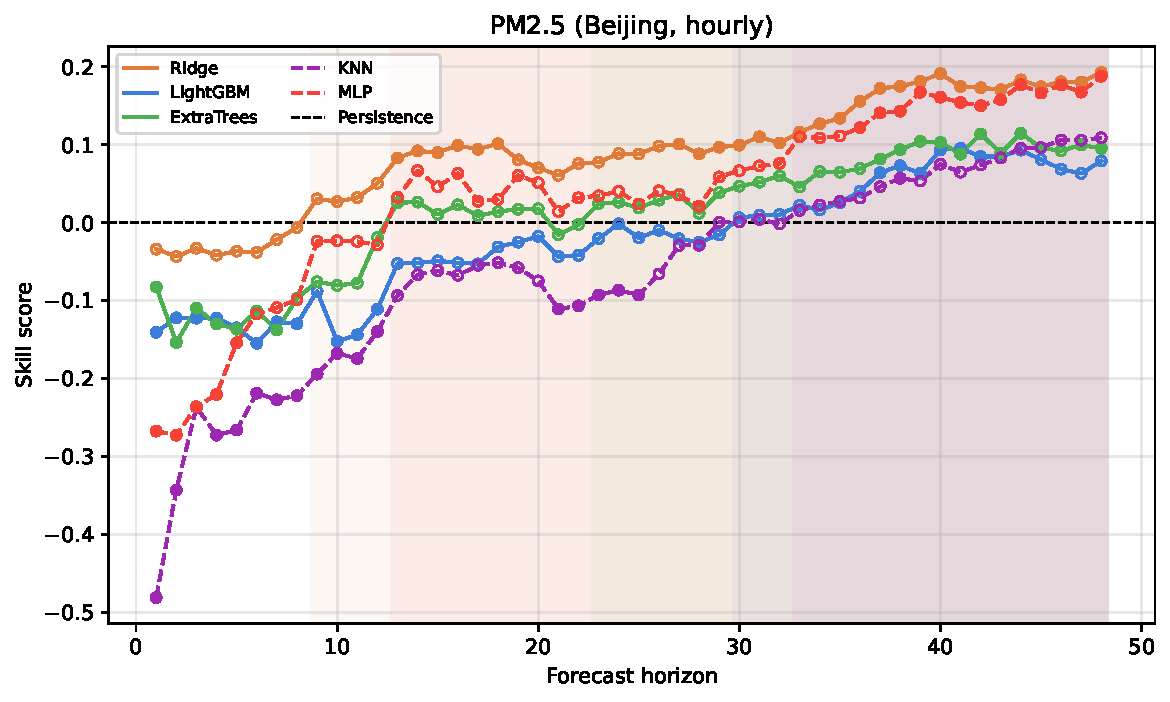
\includegraphics[width=0.88\textwidth]{fig_skill_pm25.pdf}
  \caption{Stored PM$_{2.5}$ skill curve $\mathrm{Skill}(h)$. The retained figure's horizontal axis denotes observation steps, not verified elapsed hours. Positive skill emerges late in this compressed sequence.}
  \label{fig:skill-pm25}
\end{figure}

\subsection{Electric load domain}\label{sec:load}

\subsubsection{Experimental setting}
The second domain considered is aggregate daily electricity demand, derived from the UCI Electricity Load Diagrams 2011--2014 dataset \citep{trindade2015}. This experiment uses daily observations, a persistence baseline, and the canonical comparable LightGBM protocol, with performance evaluated through MAE-based skill. The energy setting is especially informative because the series is highly regular, and persistence is expected to be particularly difficult to outperform; more broadly, electric load forecasting is a canonical operational setting where benchmarking and uncertainty-aware evaluation are central concerns \citep{hong2016}.

\subsubsection{Observed skill behavior}
Daily electric load was evaluated at horizons $h=1,\ldots,7$ days. Ridge achieves sustained positive skill across the full evaluated range, with $H^*(\mathrm{relax})=H^*(\mathrm{strict})=7$ and $[h_{\mathrm{start}},h_{\mathrm{end}}]=[1,7]$ (Table~\ref{tab:results}). By contrast, both tree-based models collapse immediately against persistence, yielding $H^*(\mathrm{relax})=H^*(\mathrm{strict})=0$. Fig.~\ref{fig:skill_load} shows the corresponding skill curves.

\subsubsection{Interpretation}
This domain illustrates that positive sample skill and statistical evidence can diverge. Although Ridge yields $H^*(\mathrm{strict})=7$ on the load series, none of its horizons has a stored DM/BH rejection (Table~\ref{tab:results}). This does not demonstrate equivalence to persistence or establish a specific explanation in terms of statistical power. Terminal-day coverage also requires verification.
\begin{figure}[t]
  \centering
  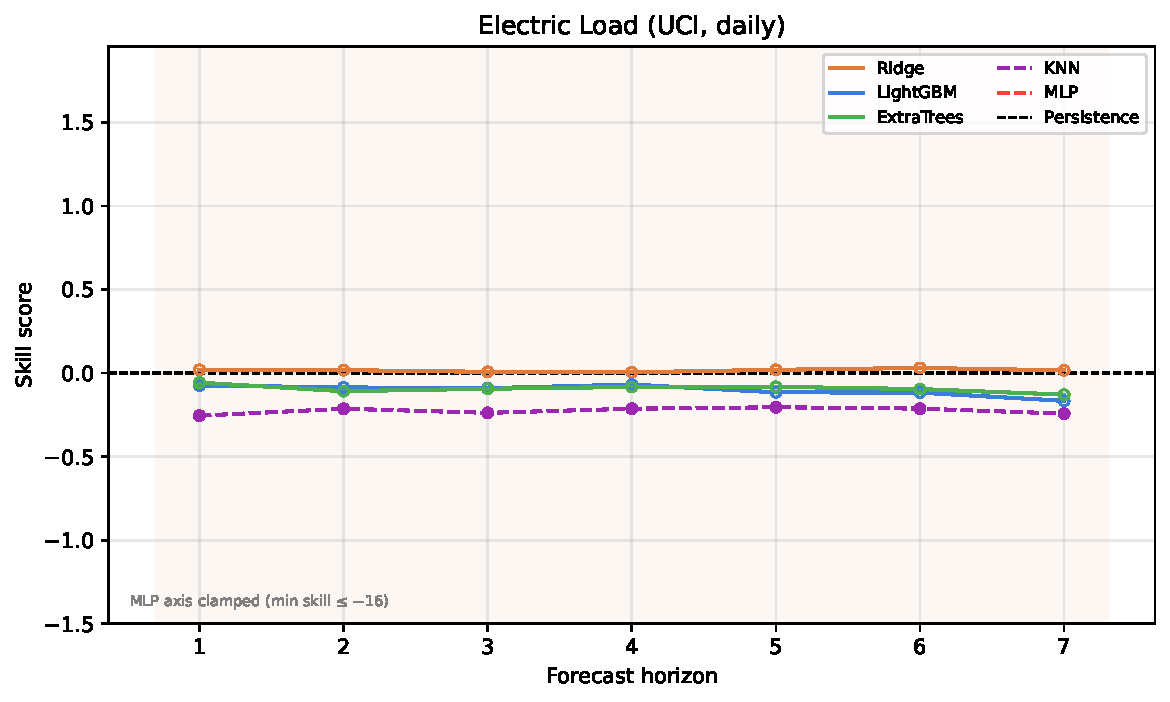
\includegraphics[width=0.88\textwidth]{fig_skill_load.pdf}
  \caption{Stored electric-load skill curve $\mathrm{Skill}(h)$ for $h=1,\ldots,7$ days. Persistence is competitive for the tree models. Absence of a stored Ridge significance rejection is not proof of equivalence or low power.}
  \label{fig:skill_load}
\end{figure}

\subsection{Wind domain}\label{sec:wind}

\subsubsection{Experimental setting}
The third domain considered is the NREL Wind Toolkit \citep{draxl2015}, which provides hourly wind-speed time series. The wind experiment uses hourly observations, a persistence baseline, and the canonical comparable LightGBM protocol under $H_{\max}=48$, with performance again evaluated through MAE-based skill. This domain is included to assess whether the proposed horizon descriptors also characterise settings in which positive skill is sustained across most or all of the evaluated horizon range.

\subsubsection{Observed skill behavior}
For wind, Ridge and LightGBM achieve sustained positive skill across the full evaluated range $h=1,\ldots,48$ (Fig.~\ref{fig:skill-wind}), yielding $H^*(\mathrm{relax})=H^*(\mathrm{strict})=48$ with $[h_{\mathrm{start}},h_{\mathrm{end}}]=[1,48]$ (Table~\ref{tab:results}). ExtraTrees is near-sustained but not fully contiguous, with $H^*(\mathrm{strict})=47$ and $[2,48]$, indicating a small short-horizon dip despite strong overall reach.

\subsubsection{Interpretation}
Wind shows sustained or nearly sustained persistence-relative skill across
the tabular models. Among the original three learners, 73--100\% of horizons
have stored two-sided DM/BH rejections (Table~\ref{tab:results}). This result
is conditional on persistence and does not establish invariance to baseline
choice or generalise beyond the sampled wind series.
\begin{figure}[t]
  \centering
  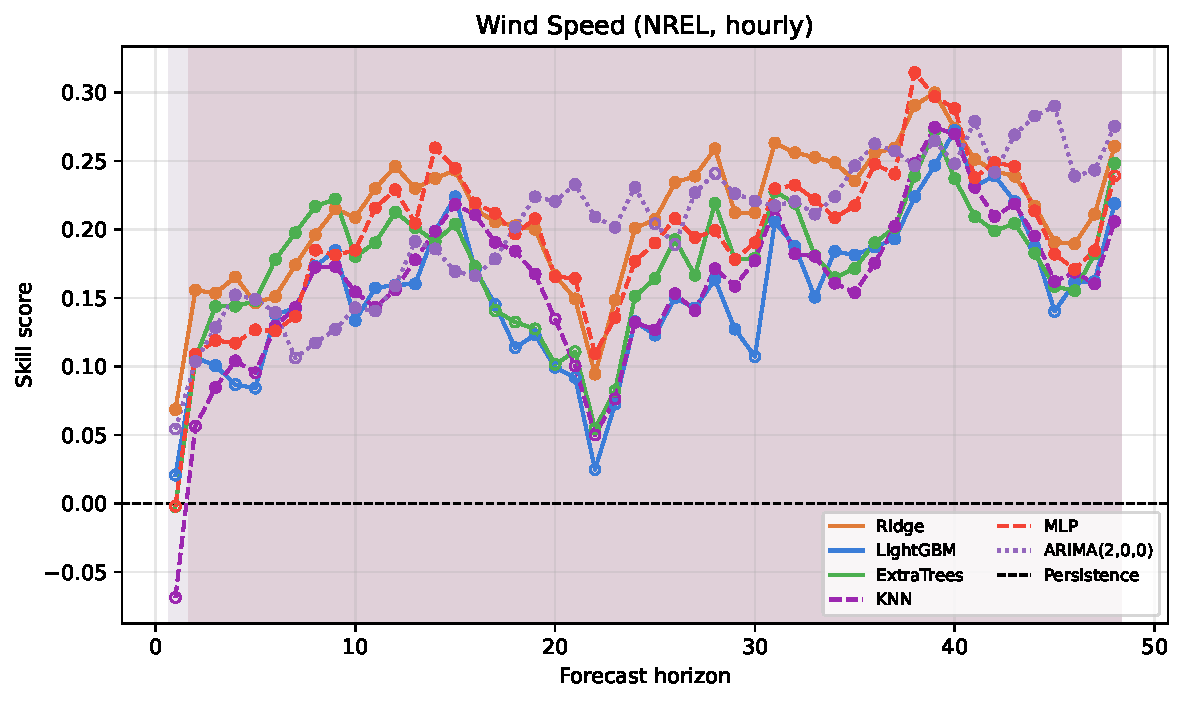
\includegraphics[width=0.88\textwidth]{fig_skill_wind.pdf}
  \caption{Wind skill curve $\mathrm{Skill}(h)$ under the leakage-free rolling-origin protocol. The skill-profile pattern shows sustained positive skill across the evaluated horizon range.}
  \label{fig:skill-wind}
\end{figure}

\subsection{Traffic domain}\label{sec:traffic}

\subsubsection{Experimental setting}
The traffic domain uses the METR-LA hourly traffic-speed dataset \citep{li2018dcrnn}. Forecasts were evaluated up to $H_{\max}=72$ under the leakage-free rolling-origin protocol, with persistence as the baseline.

\subsubsection{Observed skill behavior}
Traffic exhibits a pronounced ``ghost-skill'' pattern (Fig.~\ref{fig:skill-traffic}). For the original three models, $H^*(\mathrm{relax})=72$, but contiguous usefulness is short and occurs late in the horizon: Ridge yields $H^*(\mathrm{strict})=5$ with $[h_{\mathrm{start}},h_{\mathrm{end}}]=[63,67]$, while LightGBM and ExtraTrees yield $H^*(\mathrm{strict})=4$ with $[64,67]$ (Table~\ref{tab:results}). Stored two-sided DM/BH rejections are sparse (4--14\% of horizons); rejection direction must be read with the corresponding skill.

\subsubsection{Interpretation}
The co-occurrence of large relaxed reach and short late strict intervals indicates that most horizons are persistence-dominated, with a narrow positive cluster consistent with a daily-periodic structure in the loop-detector signal. This domain, therefore, motivates reporting $H^*(\mathrm{relax})$ and $H^*(\mathrm{strict})$ together: $H^*(\mathrm{relax})$ alone would suggest broad reach, while $H^*(\mathrm{strict})$ correctly reflects the short, isolated operational window.
\begin{figure}[t]
  \centering
  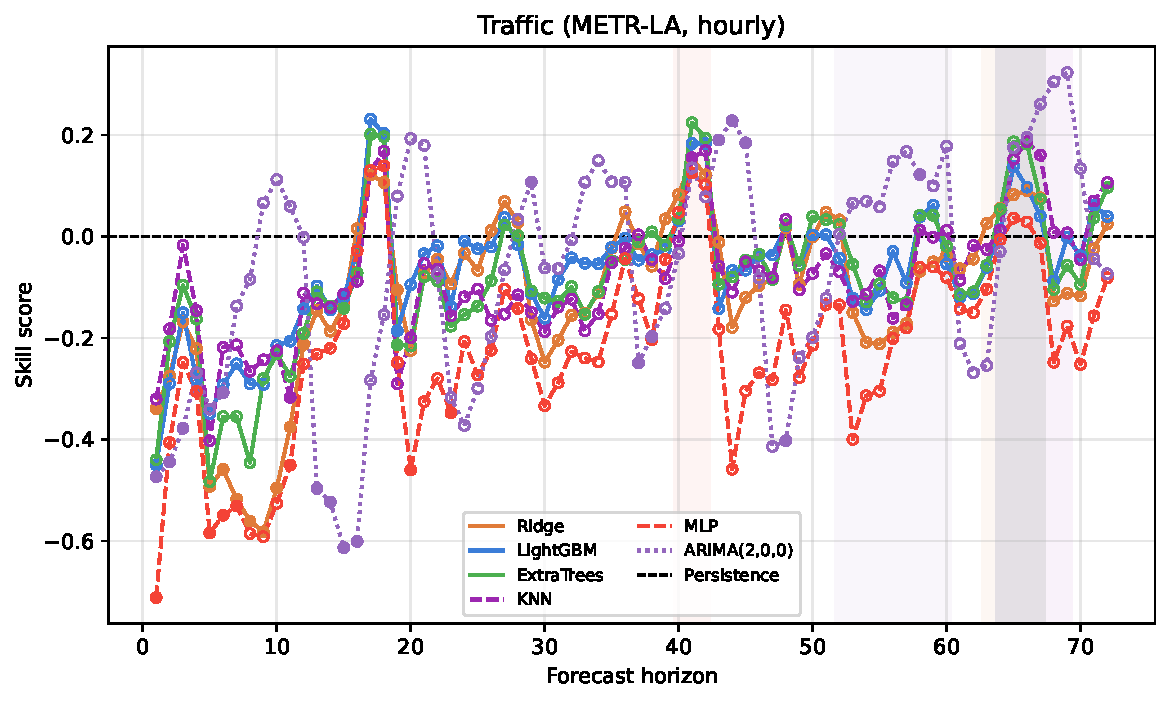
\includegraphics[width=0.88\textwidth]{fig_skill_traffic.pdf}
  \caption{Traffic skill curve $\mathrm{Skill}(h)$ under the leakage-free rolling-origin protocol. The skill-profile pattern shows fragmented positive intervals: brief, separated stretches of positive skill interspersed with negative regions.}
  \label{fig:skill-traffic}
\end{figure}

\subsection{\texorpdfstring{PM$_{10}$}{PM10} air quality domain}\label{sec:pm10}

\subsubsection{Domain overview}
The PM$_{10}$ artifacts cover Madrid Casa de Campo and Barcelona Eixample
over 2017--2024. Madrid's stored input has a complete daily axis, while
Barcelona's axis omits dates. The existing outputs use row-index horizons;
only the regular axis permits a direct conversion to days. Historical
Madrid imputation has not been shown to be causal. These retained results
are not presented as a verified cross-city deployment comparison.

\subsubsection{\texorpdfstring{PM$_{10}$}{PM10} Madrid (Casa de Campo)}
Figure~\ref{fig:skill_pm10} shows a monotone skill increase for Ridge, with $\mathrm{Skill}(h)$ rising from 0.02 at $h=1$ to 0.24 at $h=7$. Consistent with this sustained positive profile, Ridge achieves $H^*(\mathrm{relax})=H^*(\mathrm{strict})=7$ (Table~\ref{tab:results}), and 85\% of horizons are Diebold--Mariano-significant after Benjamini--Hochberg correction.
By contrast, the tree models exhibit a slight negative dip at $h=1$ (LightGBM: $-0.004$; ExtraTrees: $-0.022$) followed by sustained positive skill for $h=2,\ldots,7$. This yields \textsc{delayed\_contiguous} profiles with $H^*(\mathrm{strict})=6$ and $[h_{\mathrm{start}},h_{\mathrm{end}}]=[2,7]$, while still maintaining strong DM evidence (LightGBM: 85\%; ExtraTrees: 71\%).
\begin{figure}[t]
  \centering
  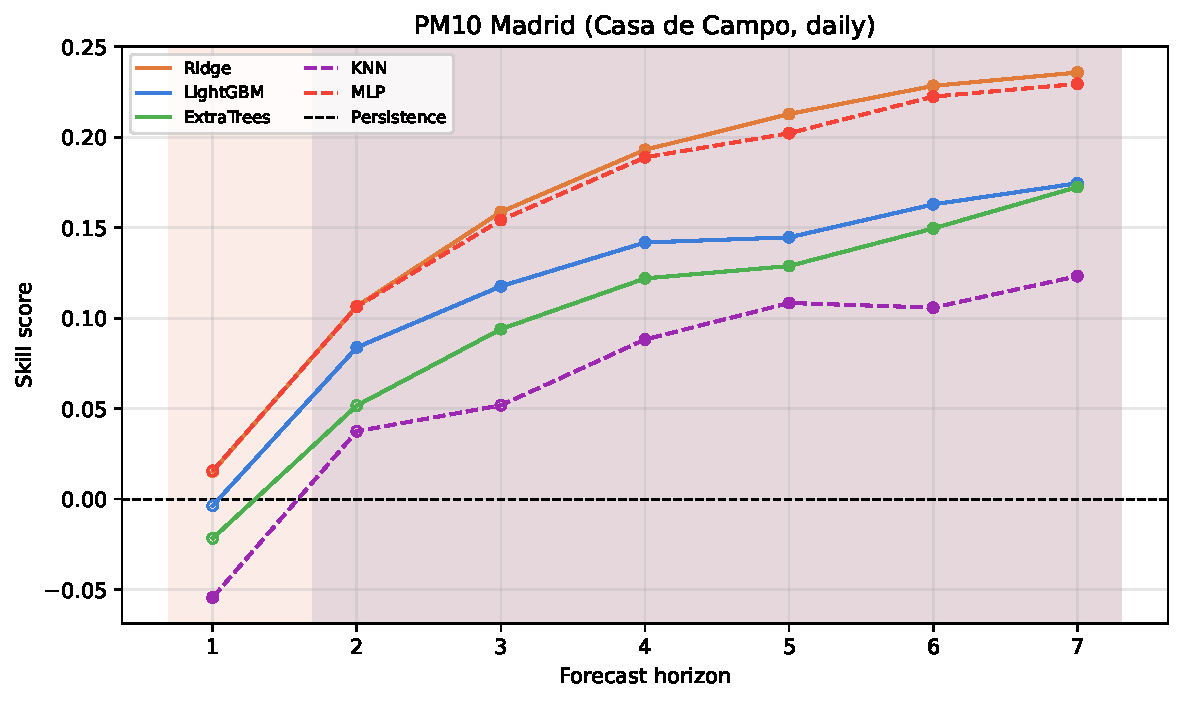
\includegraphics[width=0.88\textwidth]{fig_skill_pm10.pdf}
  \caption{Stored PM$_{10}$ (Madrid, Casa de Campo) skill curve $\mathrm{Skill}(h)$ for $h=1,\ldots,7$ days. Historical missing-value preparation is not yet verified as causal. Filled markers indicate stored BH-corrected Diebold--Mariano significance at $\alpha=0.05$; the shaded band denotes the maximizing $H^*(\mathrm{strict})$ interval.}
  \label{fig:skill_pm10}
\end{figure}

\subsubsection{\texorpdfstring{PM$_{10}$}{PM10} Barcelona (Eixample)}
In Barcelona, the original three models achieve positive skill from the
first observation step (Figure~\ref{fig:skill_pm10_bcn}), yielding
$H^*(\mathrm{relax})=H^*(\mathrm{strict})=7$ steps for Ridge, LightGBM and
ExtraTrees (Table~\ref{tab:results}). Ridge has stored rejections at 100\%
of horizons, while LightGBM and ExtraTrees each have 85\%.
Differences in baseline error between cities cannot establish an explanation
for their skill differences without controlling input preparation and elapsed
target time. We therefore make no causal attribution from this comparison.
\begin{figure}[t]
  \centering
  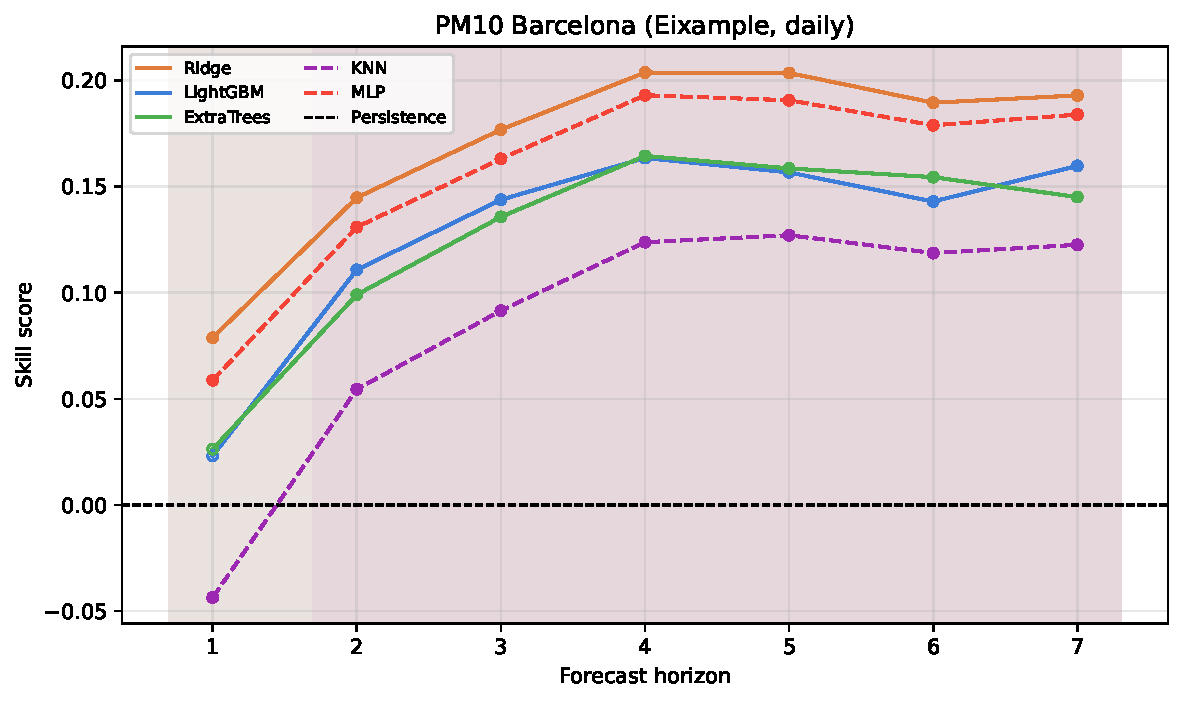
\includegraphics[width=0.88\textwidth]{fig_skill_pm10_bcn.pdf}
  \caption{PM$_{10}$ (Barcelona, Eixample) stored skill curve for $h=1,\ldots,7$ observation steps. The input omits dates, so these steps are not uniformly calendar days. Conventions otherwise match Fig.~\ref{fig:skill_pm10}.}
  \label{fig:skill_pm10_bcn}
\end{figure}

\subsubsection{Cross-city comparison}
Ridge and MLP have sustained labels in both stored PM$_{10}$ sequences.
These descriptive patterns do not establish a physical mechanism or a
validated daily alert window. Missing-date handling and historical imputation
must be checked before interpreting the difference as a cross-city effect.

Table~\ref{tab:results} reports the retained horizon descriptors and taxonomy labels for the six stored domain evaluations with persistence as baseline. Their temporal-validity limitations differ and must not be conflated with numerical reproducibility.

\begin{table}[ht]
\centering
\caption{Retained H* descriptors and stored DM significance for 30 (model, domain)
combinations. \Hrelax: last horizon with positive skill (gaps allowed).
\Hstrict: length of the longest contiguous positive-skill run.
$h_s$--$h_e$: start and end of that run.
\% DM: proportion of horizons significant at BH-corrected $\alpha=0.05$.
$\dagger$~100\,\% DM significant but \emph{worse} than persistence (negative skill).
PM$_{2.5}$ and Barcelona horizons count observations, not uniform elapsed
hours or days. Historical ARIMA results are excluded. The stored taxonomy
and BH decisions are reported with their implementation limitations.}
\label{tab:results}
\scriptsize
\setlength{\tabcolsep}{2.6pt}
\renewcommand{\arraystretch}{1.12}
\begin{tabularx}{\textwidth}{llrrrrlX}
\toprule
Domain & Model & \Hrelax & \Hstrict & $h_s$ & $h_e$ & \% DM & Profile \\
\midrule
\multirow{5}{*}{\shortstack[l]{PM$_{2.5}$\\(obs. steps)}}
  & Ridge      & 48 & 40 &  9 & 48 & 58.3\% & \textsc{fragmented} \\
  & LightGBM   & 48 & 19 & 30 & 48 & 35.4\% & \textsc{fragmented} \\
  & ExtraTrees & 48 & 26 & 23 & 48 & 37.5\% & \textsc{delayed\_contiguous} \\
  & KNN        & 48 & 16 & 33 & 48 & 37.5\% & \textsc{fragmented} \\
  & MLP        & 48 & 36 & 13 & 48 & 37.5\% & \textsc{delayed\_contiguous} \\
\midrule
\multirow{5}{*}{\shortstack[l]{Load\\(daily)}}
  & Ridge      &  7 &  7 &  1 &  7 &   0.0\%           & \textsc{sustained} \\
  & LightGBM   &  0 &  0 & ---& ---&   0.0\%           & \textsc{immediate\_collapse} \\
  & ExtraTrees &  0 &  0 & ---& ---&   0.0\%           & \textsc{immediate\_collapse} \\
  & KNN        &  0 &  0 & ---& ---& 100.0\%$^\dagger$ & \textsc{immediate\_collapse} \\
  & MLP        &  0 &  0 & ---& ---& 100.0\%$^\dagger$ & \textsc{immediate\_collapse} \\
\midrule
\multirow{5}{*}{\shortstack[l]{Wind\\(hrly)}}
  & Ridge        & 48 & 48 &  1 & 48 & 100.0\% & \textsc{sustained} \\
  & LightGBM     & 48 & 48 &  1 & 48 &  72.9\% & \textsc{sustained} \\
  & ExtraTrees   & 48 & 47 &  2 & 48 &  83.3\% & \textsc{fragmented} \\
  & KNN          & 48 & 47 &  2 & 48 &  85.4\% & \textsc{fragmented} \\
  & MLP          & 48 & 47 &  2 & 48 &  95.8\% & \textsc{fragmented} \\
\midrule
\multirow{5}{*}{\shortstack[l]{Traffic\\(hrly)}}
  & Ridge        & 72 &  5 & 63 & 67 &  13.9\% & \textsc{fragmented} \\
  & LightGBM     & 72 &  4 & 64 & 67 &   4.2\% & \textsc{fragmented} \\
  & ExtraTrees   & 72 &  4 & 64 & 67 &   4.2\% & \textsc{fragmented} \\
  & KNN          & 72 &  6 & 64 & 69 &   2.8\% & \textsc{fragmented} \\
  & MLP          & 66 &  3 & 40 & 42 &   9.7\% & \textsc{fragmented} \\
\midrule
\multirow{5}{*}{\shortstack[l]{PM10\\Madrid}}
  & Ridge      & 7 & 7 & 1 & 7 &  85.7\% & \textsc{sustained} \\
  & LightGBM   & 7 & 6 & 2 & 7 &  85.7\% & \textsc{delayed\_contiguous} \\
  & ExtraTrees & 7 & 6 & 2 & 7 &  71.4\% & \textsc{delayed\_contiguous} \\
  & KNN        & 7 & 6 & 2 & 7 &  71.4\% & \textsc{delayed\_contiguous} \\
  & MLP        & 7 & 7 & 1 & 7 &  85.7\% & \textsc{sustained} \\
\midrule
\multirow{5}{*}{\shortstack[l]{PM10\\Barcelona\\(obs. steps)}}
  & Ridge      & 7 & 7 & 1 & 7 & 100.0\% & \textsc{sustained} \\
  & LightGBM   & 7 & 7 & 1 & 7 &  85.7\% & \textsc{sustained} \\
  & ExtraTrees & 7 & 7 & 1 & 7 &  85.7\% & \textsc{sustained} \\
  & KNN        & 7 & 6 & 2 & 7 & 100.0\% & \textsc{delayed\_contiguous} \\
  & MLP        & 7 & 7 & 1 & 7 & 100.0\% & \textsc{sustained} \\
\bottomrule
\end{tabularx}
\end{table}

%% ========================================================================
%% §7 DISCUSSION
%% ========================================================================
\section{Discussion}\label{sec:discussion}

The cross-domain results in Table~\ref{tab:results} reveal that the proposed descriptors capture four qualitatively distinct skill-profile types across the six domains. This section synthesises the empirical evidence along three axes—domain versus model effects on profile type, structural periodicity as a driver of fragmented skill, and the diagnostic value of the framework at its statistical limits—and then examines what the PM$_{10}$ cross-city comparison adds to the overall picture.

\subsection{Domain drives profile type, not model class}

Table~\ref{tab:results} shows recurring descriptive patterns within the sampled
inputs. All five tabular models are labelled \textsc{sustained} or
\textsc{delayed\_contiguous} on the two PM$_{10}$ inputs and all five are
\textsc{fragmented} on Traffic. Wind reaches $H^*(\mathrm{relax})=48$ and
$H^*(\mathrm{strict})\geq47$. Both PM$_{2.5}$ and Load show variation in the
stored profile labels across models. These are descriptive labels from the
historical classification rule, not mutually exclusive physical regimes:
for example, the rule labels a near-sustained Wind profile as fragmented.

This recurrence motivates reporting interval structure alongside model
comparisons. The selected series and fixed learner configurations do not
identify a causal effect of domain dynamics or demonstrate that learner
choice is generally unimportant. The ARIMA comparison has been withdrawn
because its selection rationale and support matching were not established.

\subsection{Ghost-skill and structural periodicity in traffic}

Traffic speed has near-maximal relaxed reach (66--72 hours) across the five
tabular models but strict intervals of only 3--6 hours, located between
$h=40$ and $h=69$. This recurrence is evidence about this sensor, baseline and
protocol, not proof of a dataset-wide structural mechanism. A daily cycle is
24 observations in hourly data; 72 hours correspond to three daily cycles.
Seasonal sensitivity directly examines how the reference affects the profile.

Reporting $H^*(\mathrm{relax})=72$ alone would obscure the short continuous
windows. The five tabular models have 6--17 positive/non-positive transitions;
the full curve and interval locations therefore qualify any interpretation
of the relaxed endpoint as operational reach.

\subsection{Sensitivity to an alternative reference}\label{sec:baseline-sensitivity}
Table~\ref{tab:revision-baseline} compares persistence with seasonal persistence
using the stored LightGBM predictions on exactly the same rows. In Load,
strict continuity changes from zero to four days. In Wind it contracts from
48 hours at $[1,48]$ to 29 hours at $[20,48]$; in Traffic it expands from four
hours at $[64,67]$ to 13 hours at $[48,60]$. These changes show that baseline
sensitivity is distinct from changing the forecasting model. For hourly
endpoints that are multiples of 24, the two baselines coincide by construction;
unchanged relaxed reach at those endpoints is not independent evidence of
baseline invariance. PM$_{2.5}$ and Barcelona calendar sensitivities remain
unresolved because the frozen input axes contain gaps. The analysis neither
replaces primary results nor validates a dynamic horizon-selection controller.
% Generated values: results/dmkd_revision_audit_2026-09-30/hstar_sensitivity.csv
\begin{table}[t]
\centering
\scriptsize
\setlength{\tabcolsep}{4pt}
\begin{tabular}{@{}llrrrr@{}}
\toprule
Domain & Reference & $H^*_{\mathrm{relax}}$ & $H^*_{\mathrm{strict}}$ & $h_s$ & $h_e$ \\
\midrule
Load & Persistence & 0 & 0 & --- & --- \\
Load & Seasonal & 4 & 4 & 1 & 4 \\
Wind & Persistence & 48 & 48 & 1 & 48 \\
Wind & Seasonal & 48 & 29 & 20 & 48 \\
Traffic & Persistence & 72 & 4 & 64 & 67 \\
Traffic & Seasonal & 72 & 13 & 48 & 60 \\
\bottomrule
\end{tabular}
\caption{MAE baseline sensitivity for stored LightGBM forecasts on identical
primary support. Counts per horizon are 275--281 for Load, 350--352 for Wind,
and 102--105 for Traffic. No prediction was refitted and no row was dropped.
These are the six-domain artifact version's diagnostics; they are distinct
from the recovered four-domain revision's results.}
\label{tab:revision-baseline}
\end{table}


Fig.~\ref{fig:hstar_heatmap} visualises the contrast between \Hrelax{} and \Hstrict{} across all domains and model classes.

\begin{figure}[t]
  \centering
  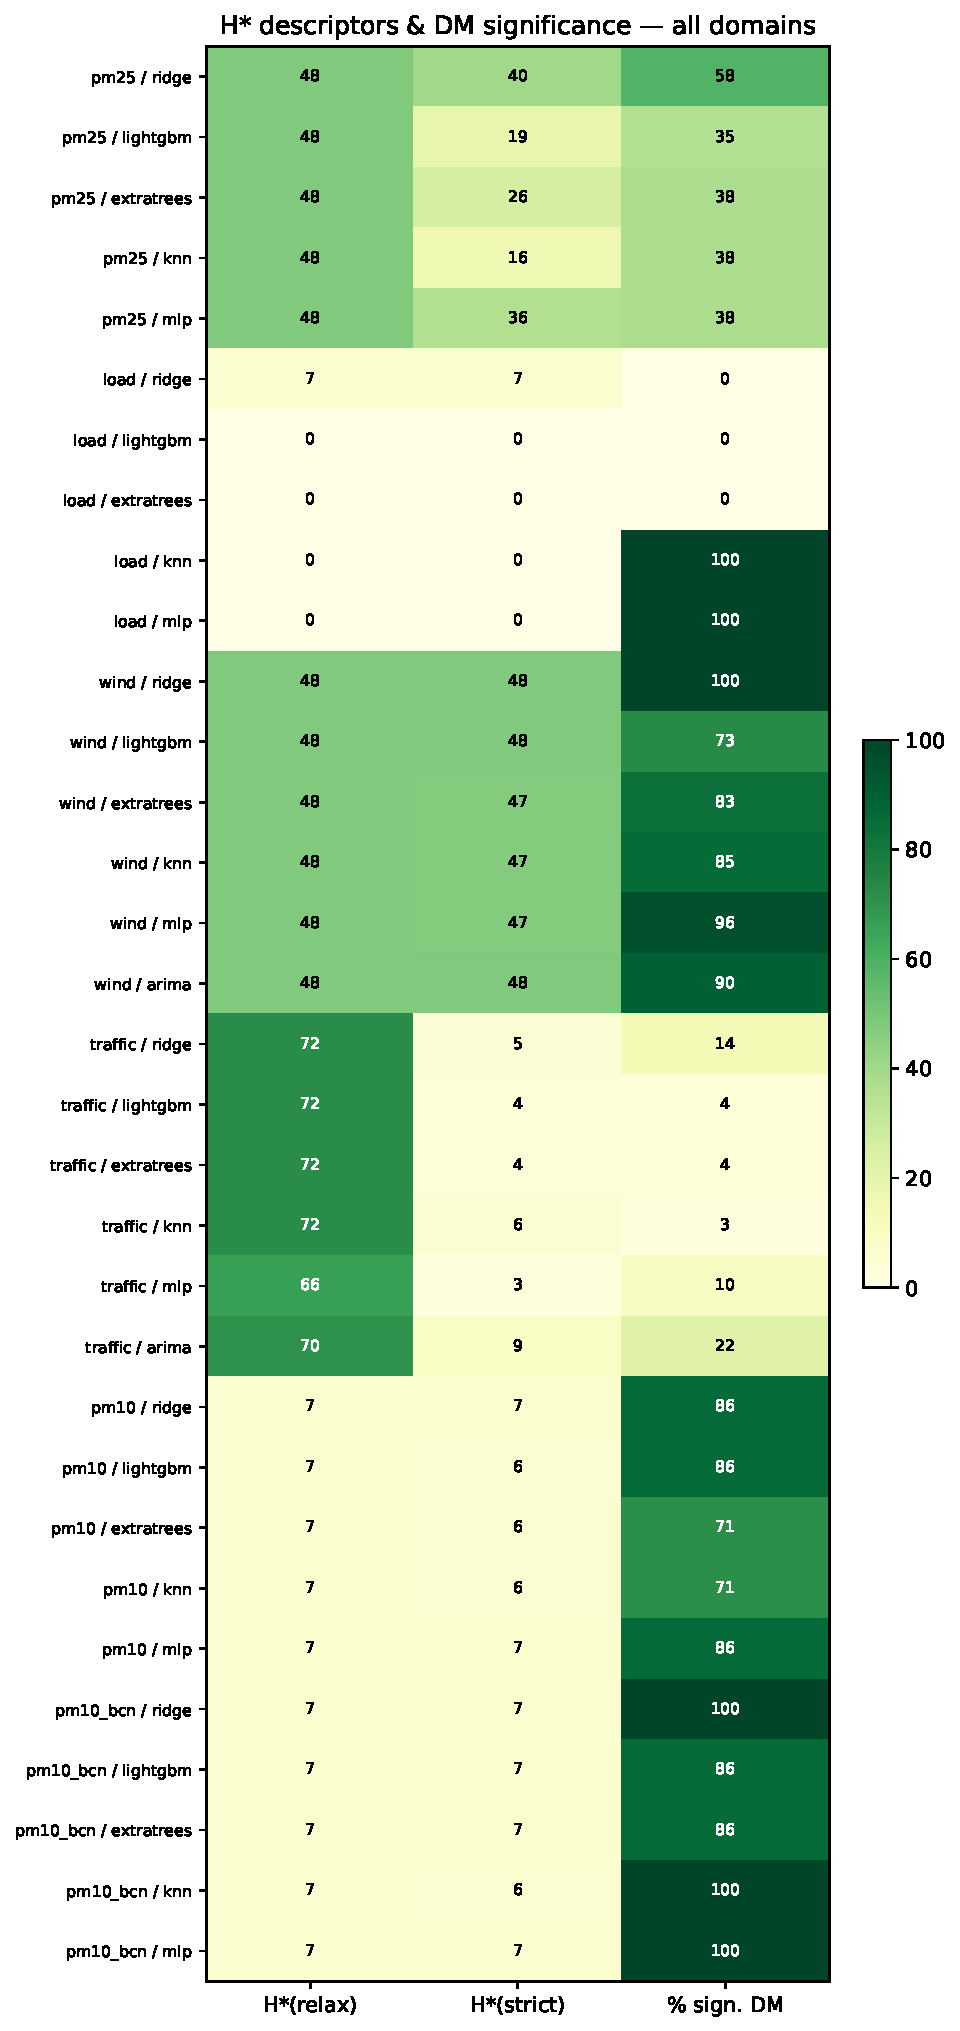
\includegraphics[width=\linewidth,height=0.62\textheight,keepaspectratio]{fig_hstar_heatmap.pdf}
  \caption{Historical \Hrelax{} and \Hstrict{} heatmap. It is retained as an
  audit artifact and includes historical ARIMA rows excluded from the revised
  comparison. PM$_{2.5}$ and Barcelona entries are observation-index
  descriptors. It must not be read as a validated calendar-time ranking.}
  \label{fig:hstar_heatmap}
\end{figure}

\subsection{Electric load as a diagnostic boundary case}

Ridge has positive point-estimate skill at all seven Load horizons but no
stored DM/BH rejection. This separates descriptive positivity from statistical
evidence. Counts vary between 275 and 281 origins. The lack of rejection does
not establish equivalence, and no quantitative power or bootstrap assertion
is made without a traceable analysis. The aggregate's unusually small final
2015-01-01 value also requires a raw interval-coverage audit before deployment
claims are warranted.

KNN and MLP have negative skill with two-sided rejections at every Load
horizon, whereas LightGBM and ExtraTrees have negative skill without stored
rejections. The MLP's large negative skill occurs on an unscaled aggregate
target. Target scaling was not changed to improve this outcome. These
observations must be read with the historical BH batch and sample-support
limitations described in the evaluation section.

Operationally, consistent deterioration argues against using a model under
that loss and support; absence of a rejection requires uncertainty assessment
and cannot by itself justify discarding or deploying a model.

\subsection{PM$_{10}$ cross-city comparison and temporal-regime sensitivity}\label{sec:pm10-discuss}

The PM$_{10}$ results at Madrid and Barcelona provide the strongest evidence for the framework's capacity to characterise sustained predictability. All ten model $\times$ station combinations are classified as \textsc{sustained} or \textsc{delayed\_contiguous}, with DM significance rates of 71--100\%. This uniformity contrasts sharply with the heterogeneity observed in the other four domains.

The stored first-step Ridge skill is 0.079 in Barcelona and 0.015 in Madrid.
The corresponding lag-1 ACF estimates are 0.644 and 0.562. This association
does not establish a causal explanation: the inputs differ in missing-day
handling and calendar support, and Barcelona's row lag is not always a
one-day lag. These differences preclude a controlled cross-city attribution.

This observation suggests that $H^*$ descriptors are sensitive to the autocorrelation regime of the target series—a property that is desirable for an operational diagnostic but that also reinforces the protocol-conditional nature of the descriptors. The mechanism connecting autocorrelation structure to skill magnitude is not pursued further in this paper, as it belongs to a different line of investigation; here, we report it as a descriptive finding that illustrates the sensitivity of the framework to domain-level temporal properties.

%% ========================================================================
%% §8 LIMITATIONS
%% ========================================================================
\section{Limitations}
The horizon descriptors reported in this paper should be interpreted as
\emph{operationally conditional} summaries rather than as universal
constants. Their values depend on the baseline choice, the maximum
evaluated horizon $H_{\max}$, dataset and domain properties, and the
evaluation design. Together, these factors determine what counts as
useful baseline-relative reach under a leakage-free protocol. This
protocol dependence is made explicit below.
More formally, the horizon descriptors reported here should be understood as
\[
H^* = H^*(\text{dataset}, \text{model}, \text{baseline}, \text{metric}, \text{validation protocol}),
\]
rather than as intrinsic properties of a forecasting system. Because both baseline competitiveness and evaluation design shape $\mathrm{Skill}(h)$, operational predictability horizons reflect an interaction of system dynamics, baseline choice, metric, and temporal validation protocol. In particular, the metric-sensitivity analysis indicates that changing the error metric from MAE to RMSE can modify not only the numerical values of $H^*(\mathrm{relax})$ and $H^*(\mathrm{strict})$ but, in some domains, the qualitative morphology of $\mathrm{Skill}(h)$ itself; consequently, claims of cross-metric invariance are not warranted in general, and any reported horizon estimates should be interpreted in the context of the full evaluation protocol.
The revised audit distinguishes train-window fitting from input preparation.
The frozen PM$_{2.5}$ sequence equals the raw non-missing subsequence exactly:
213 gaps remain after row removal, and 5,755 stored predictions have elapsed
hours different from the declared row horizon. Barcelona has 11 gaps and
1,400 predictions whose elapsed days differ from their row horizon. Calendar
forecast conclusions for these inputs therefore require a corrected regular-grid
evaluation. A sensitivity calculation on existing forecasts cannot repair that
training/target alignment. Madrid's historical missing-value preparation also
requires a causal-imputation audit. These are substantive limitations of the
retained six-domain artifacts, not just rounding or typography issues.

The numerical freeze protects reproducibility of the existing artifacts; it
does not certify their scientific interpretation. The stored DM/BH batching,
the coarse rule-based profile labels, the Load terminal-day coverage, and the
small set of fixed model configurations further restrict inference. No
prospective health-alert policy, dynamic controller, universal model
invariance or causal domain mechanism is established.
These results show why $H^*(\mathrm{relax})$ alone is not sufficient in
fragmented settings. When skill curves are non-monotonic, total positive
reach can remain stable even though contiguous usefulness and interval
structure change across models. Reporting $H^*(\mathrm{strict})$,
together with interval locations and, when needed, sign-change
structure, therefore provides a more informative summary of operational
usefulness. Clear reporting of the baseline, evaluated horizon range,
dataset, model, and protocol remains necessary for reproducibility and
for the correct interpretation of any reported $H^*$ estimate.

%% ========================================================================
%% §9 CONCLUSION
%% ========================================================================
\section{Conclusion}
This study frames predictability-horizon estimation as an operational
forecast-evaluation task, focused on skill relative to an explicit
baseline. The contribution is not a new forecasting model but a
baseline-relative way to summarise useful predictive reach
across horizons via the skill curve $\mathrm{Skill}(h)$.
Using rolling-origin evaluation against persistence, we report two
complementary horizon descriptors: $H^*(\mathrm{relax})$ (the maximum
evaluated horizon with any positive skill) and $H^*(\mathrm{strict})$
(the longest uninterrupted run of positive skill), augmented when needed
with interval locations and sign-change structure. Across the six
domains, useful predictive reach differs not only in extent but also in
continuity and fragmentation. The regular Wind and Traffic inputs show
that seasonal reference choice changes strict continuity while stored model
forecasts remain fixed. The additional PM$_{2.5}$ and PM$_{10}$ artifacts
illustrate descriptive interval patterns, but input preparation and calendar
alignment prevent unqualified calendar-time deployment conclusions. Future
work will test whether these
operational skill-profile types recur systematically across broader
domain families and evaluation designs, and whether more expressive model
classes or multivariate formulations alter the interval structure of
baseline-relative usefulness.

%% ========================================================================
%% APPENDIX
%% ========================================================================
\appendix
\subsection*{A.1 Metric sensitivity}\label{sec:metric-sensitivity}
MAE and RMSE were aggregated from the same stored per-origin predictions,
with all forecast rows and persistence values unchanged. No models were
retrained. The complete five-model diagnostics and input/output hashes are
provided in the replication audit; Table~\ref{tab:revision-rmse} shows
LightGBM for a compact comparison.

For Load, RMSE yields $H^*(\mathrm{relax})=H^*(\mathrm{strict})=2$ with
interval $[1,2]$, while MAE yields no positive horizon. For Traffic, RMSE
yields $72/53$ at $[20,72]$, compared with $72/4$ at $[64,67]$ under MAE.
Wind remains $48/48$ at $[1,48]$. The PM$_{2.5}$ sequence gives $48/19$
at $[30,48]$ under both losses; its sign-change count changes from one to
three, and its axis remains observation-based. These current results replace
the incompatible numerical claims inherited from an earlier experiment.
Madrid changes from $7/6$ to $7/7$ for LightGBM, and Barcelona remains
$7/7$ observation steps. These diagnostics address loss sensitivity only;
they cannot establish temporal validity or validate historical imputation.
% Generated values: results/dmkd_revision_audit_2026-09-30/hstar_sensitivity.csv
\begin{table}[t]
\centering
\scriptsize
\setlength{\tabcolsep}{4pt}
\begin{tabular}{@{}llrrrr@{}}
\toprule
Domain / horizon unit & Loss & $H^*_{\mathrm{relax}}$ & $H^*_{\mathrm{strict}}$ & $h_s$ & $h_e$ \\
\midrule
PM$_{2.5}$ / observed steps & MAE & 48 & 19 & 30 & 48 \\
PM$_{2.5}$ / observed steps & RMSE & 48 & 19 & 30 & 48 \\
Load / days & MAE & 0 & 0 & --- & --- \\
Load / days & RMSE & 2 & 2 & 1 & 2 \\
Wind / hours & MAE & 48 & 48 & 1 & 48 \\
Wind / hours & RMSE & 48 & 48 & 1 & 48 \\
Traffic / hours & MAE & 72 & 4 & 64 & 67 \\
Traffic / hours & RMSE & 72 & 53 & 20 & 72 \\
PM$_{10}$ Madrid / days & MAE & 7 & 6 & 2 & 7 \\
PM$_{10}$ Madrid / days & RMSE & 7 & 7 & 1 & 7 \\
PM$_{10}$ Barcelona / observed steps & MAE & 7 & 7 & 1 & 7 \\
PM$_{10}$ Barcelona / observed steps & RMSE & 7 & 7 & 1 & 7 \\
\bottomrule
\end{tabular}
\caption{LightGBM metric sensitivity with persistence on unchanged forecast
support. Observation steps are not necessarily uniform calendar intervals.
The complete five-model results are provided in the revision audit.}
\label{tab:revision-rmse}
\end{table}


%% ========================================================================
%% DECLARATIONS
%% ========================================================================
\section*{Declarations}
\subsection*{Funding}
The authors did not receive support from any organisation for the submitted work.
\subsection*{Competing Interests}
The authors declare that there are no relevant financial or non-financial competing interests to disclose.
\subsection*{Ethics Approval}
Not applicable. This study is based exclusively on publicly available benchmark datasets. It did not involve human participants, animals, patient data, or primary data collection.
\subsection*{Data Availability}
The local replication package has a single data entry point,
\texttt{data/README.md}, and a machine-readable checksum manifest,
\texttt{data/MANIFEST.tsv}. Exact processed inputs are assembled into one
local archive for review. Public release of that archive has not yet been
verified, and it must not be claimed that every input is already cached in
the public repository. Wind and Traffic retrieval instructions are retained
in the recovered four-domain revision package. The original sources are:
\begin{itemize}
  \item \textbf{PM$_{2.5}$:} Beijing PM$_{2.5}$ dataset \citep{chen2015beijingpm25}, UCI Machine Learning Repository, \url{https://doi.org/10.24432/C5JS49}.
  \item \textbf{Electric Load:} UCI Electricity Load Diagrams 2011--2014 \citep{trindade2015}, \url{https://doi.org/10.24432/C58C86}.
  \item \textbf{Wind:} NREL Wind Integration National Dataset (WIND) Toolkit \citep{draxl2015}, distributed by the National Renewable Energy Laboratory.
  \item \textbf{Traffic:} METR-LA dataset \citep{li2018dcrnn}; the processed file (\texttt{metr-la.h5}) was obtained from the public data links in the original DCRNN repository.
  \item \textbf{PM$_{10}$ Madrid and Barcelona:} Daily PM$_{10}$ concentrations from the Spanish air quality monitoring network, stations Casa de Campo (Madrid) and Eixample (Barcelona, code 08019043), 2017--2024. Data publicly available from the Ministerio para la Transici\'on Ecol\'ogica y el Reto Demogr\'afico (MITECO) and the Catalan air quality service (Xarxa de Vigil\`ancia i Previsi\'o de la Contaminaci\'o Atmosf\`erica, XVPCA).
\end{itemize}
\subsection*{Code Availability}
The evaluation scripts, rolling-origin evaluator, $H^*$ computation, and Diebold--Mariano testing code are available in the project repository: \url{https://github.com/EduIntellect/paper2H}.

\section*{Acknowledgments}
None.

% Springer/DMKD bibliography (BibTeX)
\bibliographystyle{sn-basic}
\bibliography{sn-bibliography}
\end{document}
